% !TEX root = ./correctness-deciders.tex
\title{Correctness of bbchallenge's deciders}
\author{
        Tristan St\'{e}rin
}

\documentclass[a4paper,british]{article}
\usepackage{babel}
\usepackage[utf8]{inputenc}
\usepackage[margin=1in]{geometry}
%\usepackage{subfig}
\usepackage[hidelinks]{hyperref}
\usepackage{subcaption} 
\usepackage{tikz}

\usepackage{algorithm}
\usepackage[noend]{algpseudocode}

\usepackage{graphicx}

\usepackage{amsmath,amsfonts,amssymb,amsthm}


\newtheorem{theorem}{Theorem}
\newtheorem{definition}[theorem]{Definition}
\newtheorem{lemma}[theorem]{Lemma}
\newtheorem{proposition}[theorem]{Proposition}
\newtheorem{corollary}[theorem]{Corollary}

\newtheorem{observation}[theorem]{Observation}
\newtheorem{example}[theorem]{Example}
\newtheorem{remark}[theorem]{Remark}


\usepackage{microtype,xspace,wrapfig,multicol} 
\usepackage[textsize=tiny,color=lightgray]{todonotes} 
\usepackage[normalem]{ulem} % sout

\newcommand{\ts}[1]{{\color{red}#1}}
\newcommand{\tsi}[1]{\todo[inline]{TS: #1}}
\newcommand{\tsm}[1]{\todo{TS: #1}}
\newcommand{\tss}[2]{{\ts{\sout{#1}}} {\ts{#2}}}
\newcommand{\tabi}{\hspace{\algorithmicindent}}

\usepackage{xcolor}

\definecolor{colorA}{RGB}{255,0,0}
\definecolor{colorB}{RGB}{255,128,0}
\definecolor{colorC}{RGB}{0,0,255}
\definecolor{colorD}{RGB}{0,255,0}
\definecolor{colorE}{RGB}{255,0,255}

\begin{document}
\date{}
\maketitle

\begin{abstract}
        The Busy Beaver Challenge (or bbchallenge) aims at collaboratively solving the following conjecture: ``BB(5) = 47,176,870'' [Aaronson, 2020]\nocite{BusyBeaverFrontier}. This goal amounts to decide whether or not 88,664,064 Turing machines with 5-state halt or not -- starting from all-0 tape. In order to decide the behavior of these machines we write \textit{deciders}. A decider is a program that takes as input a Turing machine and outputs \texttt{true} if it is able to tell whether the machine halts or not. Each decider is specialised in recognising a particular type of behavior that can be decided. 
        
        In this document we are concerned with proving the correctness of these deciders programs. More context and information about this methodology are available at \url{https://bbchallenge.org}.
\end{abstract}
\tableofcontents

\section{Conventions}

\begin{table}[h!]
  \centering
  \begin{tabular}{lll}
    & 0   & 1   \\
  A & 1RB & 1LC \\
  B & 1RC & 1RB \\
  C & 1RD & 0LE \\
  D & 1LA & 1LD \\
  E & - - - & 0LE
  \end{tabular}
  \caption{Transition table of the current 5-state busy beaver champion: it halts after 47,176,870 steps.\\\url{https://bbchallenge.org/1RB1LC1RC1RB1RD0LE1LA1LD---0LA&status=halt}}
  \end{table}\label{table:bb5}

The set $\mathbb{N}$ denotes $\{0,1,2\dots\}$. 

\paragraph*{Turing machines.}The Turing machines that are studied in the context of bbchallenge use a binary alphabet and a single bi-infinite tape. Machine transitions are either undefined (in which case the machine halts) or given by (a) a symbol to write (b) a direction to move (left or right) and (c) a state to go to. Table~\ref{table:bb5} gives the transition table of the current 5-state busy beaver champion. The machine halts after 47,176,870 steps (starting from all-0 tape) when it reads a 0 in state E, which is undefined.

A \textit{configuration} of a Turing machine is defined by the 3-tuple: (i) state (ii) position of the head (iii) content of the memory tape. In the context of bbchallenge, \textit{the initial configuration} of a machine is always (i) state is 0, i.e. the first state to appear in the machine's description (ii) head's position is 0 (iii) the initial tape is all-0 -- i.e. each memory cell is containing 0. We write $c_1 \vdash_\mathcal{M} c_2$ if a configuration $c_2$ is obtained from $c_1$ in one computation step of machine $\mathcal{M}$. We omit $\mathcal{M}$ if it is clear from context. We let $c_1 \vdash^s c_2$ denote a sequence of $s$ computation steps, and let  $c_1 \vdash^* c_2$ denote zero or more computation steps. % exact same wording as in https://dna.hamilton.ie/assets/dw/NearyWoodsFCT09.pdf
We write $c_1 \vdash \bot$ if the machine halts after executing one computation step from configuration $c_1$. In the context of bbchallenge, halting happens when an undefined machine transition  is met i.e. no instruction is given for when the machine is in the state, tape position and tape corresponding to configuration $c_1$.

\paragraph*{Space-time diagram.} We use space-time diagrams to give a visual representation of the behavior of a given machine. The space-time diagram of machine $\mathcal{M}$ is an image where the $i^\text{th}$ row of the image gives:
\begin{enumerate}
  \item The content of the tape after $i$ steps (black is 0 and white is 1).
  \item The position of the head is colored to give state information using the following colours for 5-state machines: \textcolor{colorA}{A},  \textcolor{colorB}{B},  \textcolor{colorC}{C},  \textcolor{colorD}{D},  \textcolor{colorE}{E}.
\end{enumerate}

\section{Decider for ``Cyclers''}\label{sec:cyclers}

\begin{figure}[h!]
\centering

\includegraphics[width=0.4\textwidth]{space-time-diagrams/cycler_279081.pdf}
\hspace{2ex}
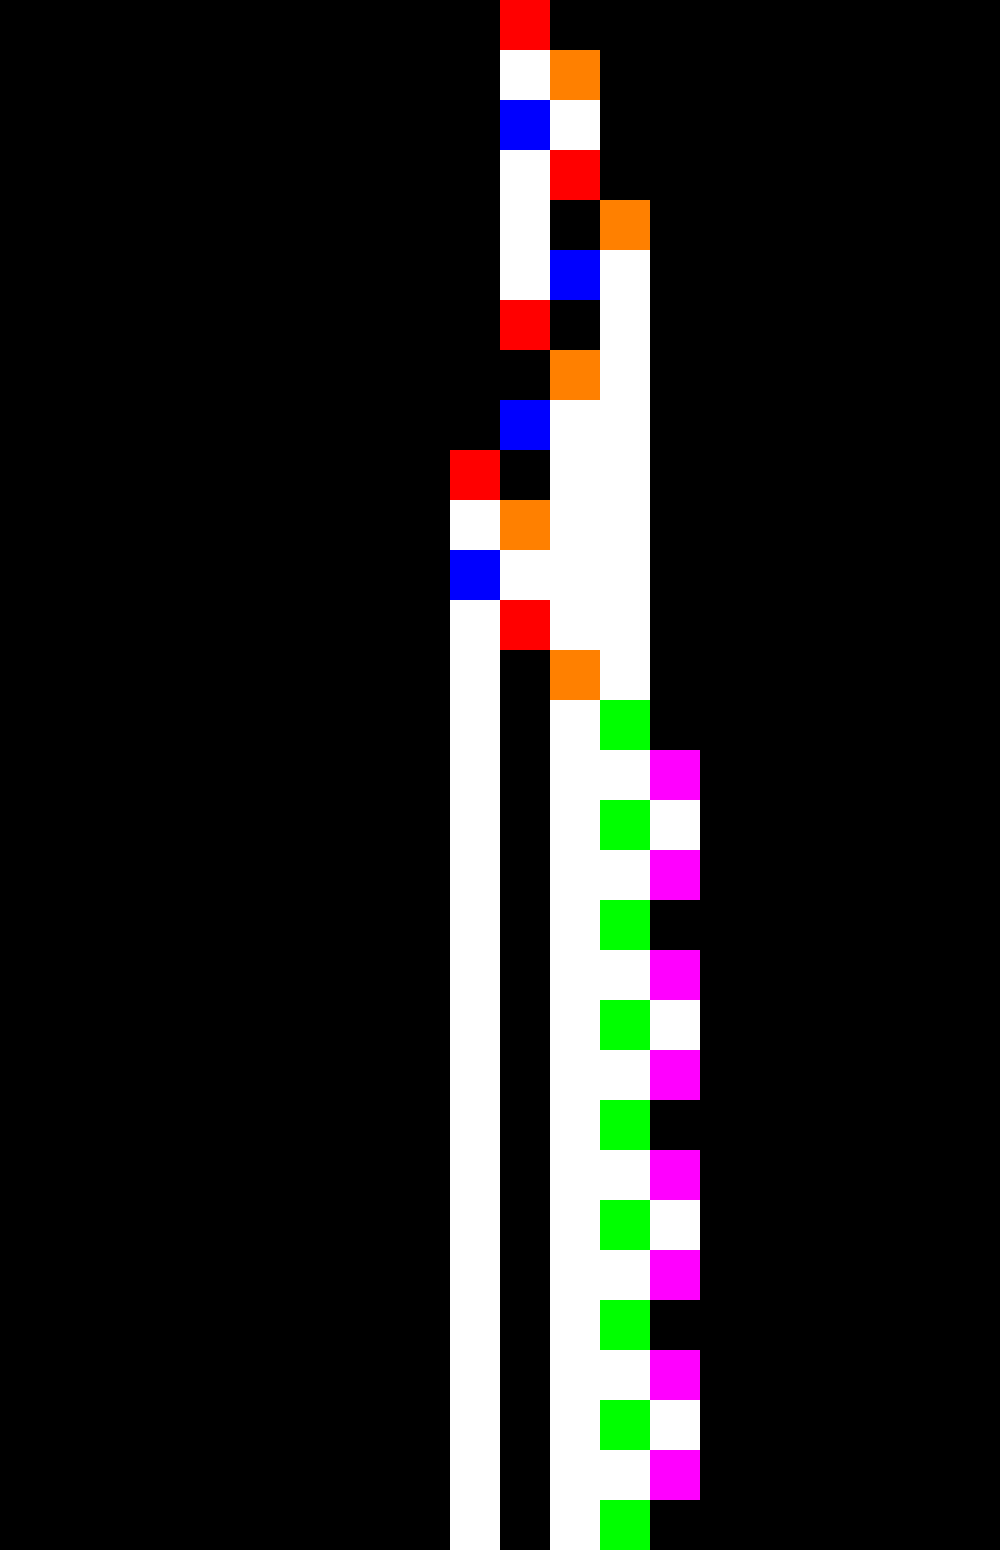
\includegraphics[width=0.4\textwidth]{space-time-diagrams/cycler_4239083.pdf}
\caption{Space-time diagrams of the 30 first steps of bbchallenge's machines \#279,081 (left) and \#4,239,083 (right) which are both ``Cyclers'': they eventually repeat the same configuration for ever. \\
Access the machines at \url{https://bbchallenge/279081} and 
\url{https://bbchallenge/4239083}.}\label{fig:cyclers}
\end{figure}

The goal of this decider is to recognise Turing machines that cycle through the same configurations for ever. Such machines never halt. The method is simple: remember every configuration seen by a machine and return \texttt{true} if one is visited twice. A time limit (maximum number of steps) is also given for running the test in practice: the algorithm recognises any machine whose cycle fits within this limit\footnote{In practice, for machines with 5 states the decider was run with 1000 steps time limit.}.


\begin{example}\normalfont
Figure~\ref{fig:cyclers} gives the space-time diagrams of the 30 first iterations of two ``Cyclers'' machines: bbchallenge's machines \#279,081 (left) and \#4,239,083 (right). Refer to \url{https://bbchallenge/279081} and 
\url{https://bbchallenge/4239083} for their transition tables. From these space-time diagrams we see that the machines eventually repeat the same configuration.
\end{example}

\newpage
\subsection{Pseudocode}

We assume that we are given a Turing Machine type \textbf{TM} that encodes the transition table of a machine as well as a procedure \textbf{TuringMachineStep}(machine,configuration) which computes the next configuration of a Turing machine from the given configuration or \textbf{nil} if the machine halts at that step.

\begin{algorithm}
        \caption{{\sc decider-cylers}}\label{alg:cyclers}

        \begin{algorithmic}[1]

                \State \textbf{struct} Configuration \{
                \State \tabi\textbf{int} state
                \State \tabi\textbf{int} headPosition
                \State \tabi\textbf{int $\boldsymbol{\to}$ int} tape
                \State \}
                \State 
                \Procedure{\textbf{bool} {\sc decider-cylers}}{\textbf{TM} machine,\textbf{int} timeLimit}
                \State \textbf{Configuration} currConfiguration = \{.state = 0,$\,$.headPosition = 0,$\,$ .tape = \{0:0\}\}
                \State \textbf{Set$\boldsymbol{<}$Configuration$\boldsymbol{>}$} configurationsSeen = \{\}
                \State \textbf{int} currTime = 0

                \While{currTime $<$ timeLimit}
                \If{currConfiguration \textbf{in} configurationsSeen}
                \State \textbf{return} true
                \EndIf
                \State configurationsSeen.\textbf{insert}(currConfiguration)

                \State currConfiguration = \textbf{TuringMachineStep}(machine,currConfiguration)
                \State currTime += 1


                \If{currConfiguration == \textbf{nil}}
                \State \textbf{return} false //machine has halted, it is not a Cycler
                \EndIf
                \EndWhile

                \State \textbf{return} false
                \EndProcedure

        \end{algorithmic}
\end{algorithm}

\subsection{Correctness}



\begin{theorem}\label{th:cyclers}\normalfont Let $\mathcal{M}$ be a Turing machine and $t \in \mathbb{N}$ a time limit. Let $c_0$ be the initial configuration of the machine. There exists $i\in\mathbb{N}$ and $j\in\mathbb{N}$ such that $c_0 \vdash^i c_i \vdash^j c_i$ with $i+j \leq t$ if and only if {\sc decider-cyclers}($\mathcal{M}$,$t$) returns \texttt{true} (Algorithm~\ref{alg:cyclers}).
\end{theorem}
\begin{proof}
        This follows directly from the behavior of {\sc decider-cyclers}($\mathcal{M}$,$t$): all intermediate configurations below time $t$ are recorded and the algorithm returns \texttt{true} if and only if one is visited twice. This mathematically translates to
        there exists $i\in\mathbb{N}$ and $j\in\mathbb{N}$ such that $c_0 \vdash^i c_i \vdash^j c_i$ with $i+j \leq t$, which is what we want. Index $i$ corresponds to the first time that $c_i$ is seen (l.13 in Algorithm~\ref{alg:cyclers}) while index $j$ corresponds to the second time that $c_i$ is seen (l.11 in Algorithm~\ref{alg:cyclers}).
\end{proof}

\begin{corollary}\normalfont
        Let $\mathcal{M}$ be a Turing machine and $t \in \mathbb{N}$ a time limit. If {\sc decider-cyclers}($\mathcal{M}$,$t$) returns \texttt{true} then the behavior of $\mathcal{M}$ from all-0 tape has been decided: $\mathcal{M}$ does not halt.
\end{corollary}
\begin{proof}
        By Theorem~\ref{th:cyclers}, there exists $i\in\mathbb{N}$ and $j\in\mathbb{N}$ such that $c_0 \vdash^i c_i \vdash^j c_i$ with $i+j \leq t$. It follows that for all $k\in\mathbb{N}$, $c_0 \vdash^{i+kj} c_i$. The machine never halts as it will visit $c_i$ infinitely often.
\end{proof}

\subsection{Results}

The decider was coded in \texttt{golang} and is accessible at this link: \url{https://github.com/bbchallenge/bbchallenge-deciders/tree/main/decider-cyclers}.

The decider found 11,229,238 ``Cyclers'', out of 88,664,064 machines in the seed database of the Busy Beaver Challenge (c.f. \url{https://bbchallenge.org/method#seed-database}). More information about these results are available at: \url{https://discuss.bbchallenge.org/t/decider-cyclers/33}.


\bibliographystyle{abbrv}
\bibliography{correctness-deciders}

\end{document}